\chapter{Clustering}


\section{Similarity and dissimilarity}

\begin{description}
    \item[Similarity] \marginnote{Similarity}
        Measures how alike two objects are.
        Often defined in the range $[0, 1]$.

    \item[Dissimilarity] \marginnote{Dissimilarity}
        Measures how two objects differ.
        0 indicates no difference while the upper bound varies.
\end{description}

\begin{table}[H]
    \centering
    \renewcommand{\arraystretch}{2}
    \begin{tabular}{c | c | c}
        \textbf{Attribute type} & \textbf{Dissimilarity} & \textbf{Similarity} \\
        \hline
        Nominal & $d(p, q) = \begin{cases} 0 & \text{if } p=q \\ 1 & \text{if } p \neq q \end{cases}$ & $s(p, q) = 1 - d(p, q)$ \\
        \hline
        Ordinal & $d(p, q) = \frac{\vert p - q \vert}{V}$ with $p, q \in \{ 0, \dots, V \}$ & $s(p, q) = 1 - d(p, q)$ \\
        \hline
        Interval or ratio & $d(p, q) = \vert p - q \vert$ & $s(p, q) = \frac{1}{1 + d(p, q)}$
    \end{tabular}
    \caption{Similarity and dissimilarity by attribute type}
\end{table}

\begin{description}
    \item[Similarity properties] \phantom{}
        \begin{enumerate}
            \item $\texttt{sim}(p, q) = 1$ iff $p = q$. 
            \item $\texttt{sim}(p, q) = \texttt{sim}(q, p)$. 
        \end{enumerate}
\end{description}


\subsection{Distance}

Given two $D$-dimensional data entries $p$ and $q$, possible distance metrics are:
\begin{descriptionlist}
    \item[Minkowski distance ($L_r$)] \marginnote{Minkowski distance}
        \[ \texttt{dist}(p, q) = \left( \sum_{d=1}^{D} \vert p_d - q_d \vert^r \right)^{\frac{1}{r}} \]
        where $r$ is a parameter.

        Common values for $r$ are:
        \begin{descriptionlist}
            \item[$r = 1$] 
                Corresponds to the $L_1$ norm.
                It is useful for discriminating 0 distance and near-0 distance as 
                an $\varepsilon$ change in the data corresponds to an $\varepsilon$ change in the distance.
            \item[$r = 2$]
                Corresponds to the Euclidean distance or $L_2$ norm.
            \item[$r = \infty$]
                Corresponds to the $L_\infty$ norm.
                Considers only the dimensions with the maximum difference.
        \end{descriptionlist}
    
    \item[Mahalanobis distance] \marginnote{Mahalanobis distance}
        \[ \texttt{dist}(p, q) = \sqrt{ (p-q) \matr{\Sigma}^{-1} (p-q)^T } \]
        where $\matr{\Sigma}$ is the covariance matrix of the dataset.
        The Mahalanobis distance of $p$ and $q$ increases when the segment connecting them 
        points towards a direction of greater variation of the data.

        \begin{figure}[H]
            \centering
            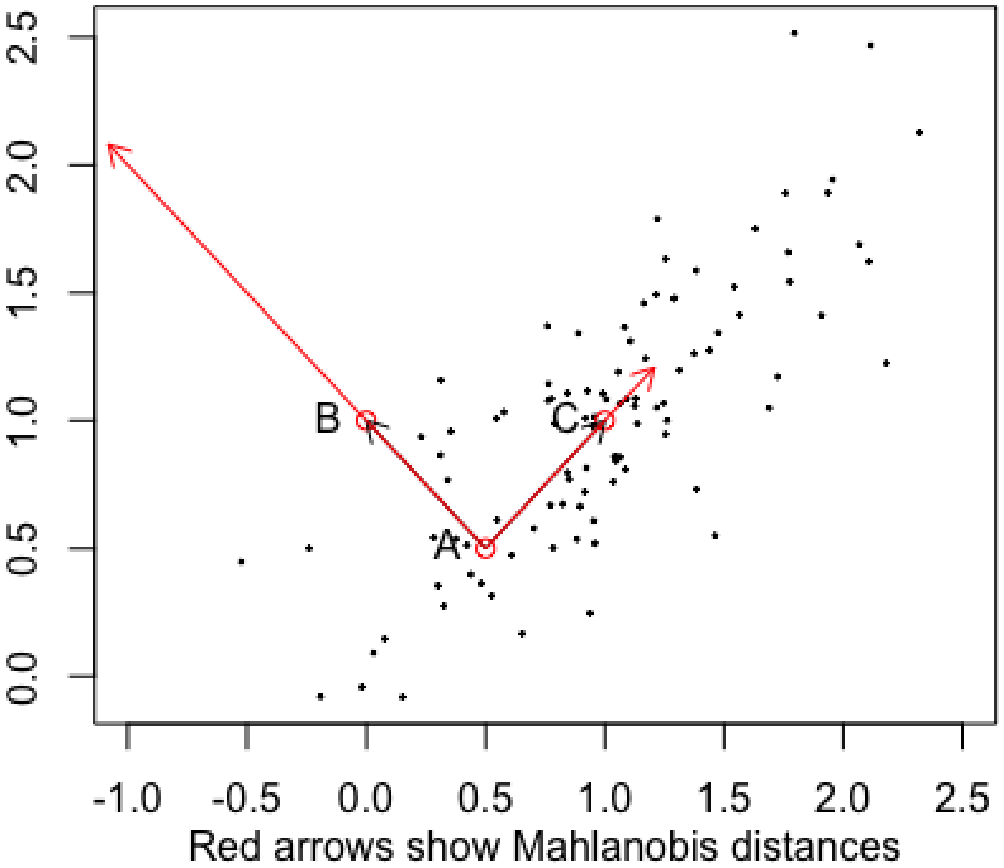
\includegraphics[width=0.35\textwidth]{img/mahalanobis.png}
            \caption{The Mahalanobis distance between $(A, B)$ is greater than $(A, C)$, while the Euclidean distance is the same.}
        \end{figure}
\end{descriptionlist}

\subsubsection{Distance properties}
\begin{descriptionlist}
    \item[Positive definiteness] 
        $\texttt{dist}(p, q) \geq 0$ and $\texttt{dist}(p, q) = 0$ iff $p = q$.
    \item[Symmetry] 
        $\texttt{dist}(p, q) = \texttt{dist}(q, p)$
    \item[Triangle inequality] 
        $\texttt{dist}(p, q) \leq \texttt{dist}(p, r) + \texttt{dist}(r, q)$
\end{descriptionlist}



\subsection{Vector similarity}

\begin{description}
    \item[Binary vectors]
        Given two examples $p$ and $q$ with binary features, we can compute the following values:
        \[ 
            \begin{split}
                M_{00} &= \text{ number of features that equals to 0 for both $p$ and $q$} \\
                M_{01} &= \text{ number of features that equals to 0 for $p$ and 1 for $q$} \\
                M_{10} &= \text{ number of features that equals to 1 for $p$ and 0 for $q$} \\
                M_{11} &= \text{ number of features that equals to 1 for both $p$ and $q$}
            \end{split}    
        \]
        Possible distance metrics are:
        \begin{descriptionlist}
            \item[Simple matching coefficient] \marginnote{Simple matching coefficient}
                $\texttt{SMC}(p, q) = \frac{M_{00} + M_{11}}{M_{00} + M_{01} + M_{10} + M_{11}}$ 
            \item[Jaccard coefficient] \marginnote{Jaccard coefficient}
                $\texttt{JC}(p, q) = \frac{M_{11}}{M_{01} + M_{10} + M_{11}}$ 
        \end{descriptionlist}

    \item[Cosine similarity] \marginnote{Cosine similarity}
        Cosine of the angle between two vectors:
        \[ \texttt{cos}(p, q) = \frac{p \cdot q}{\Vert p \Vert \cdot \Vert q \Vert} \]

    \item[Extended Jaccard coefficient (Tanimoto)] \marginnote{Extended Jaccard coefficient (Tanimoto)}
        Variation of the Jaccard coefficient for continuous values:
        \[ \texttt{T}(p, q) = \frac{p \cdot q}{\Vert p \Vert^2 + \Vert q \Vert^2 - p \cdot q} \]
\end{description}


\subsection{Correlation}

\begin{description}
    \item[Pearson's correlation] \marginnote{Pearson's correlation}
        Measure of linear relationship between a pair of quantitative attributes $e_1$ and $e_2$.
        To compute Pearson's correlation, the values of $e_1$ and $e_2$ are first standardized and then ordered to obtain the vectors $\vec{e}_1$ and $\vec{e}_2$.
        The correlation is then computed as the dot product between $\vec{e}_1$ and $\vec{e}_2$:
        \[ \texttt{corr}(e_1, e_2) = \langle \vec{e}_1, \vec{e}_2 \rangle \]

        Pearson's correlation has the following properties:
        \begin{itemize}
            \item If the variables are independent, then the correlation is 0 (but not vice versa).
            \item If the correlation is 0, then there is no linear relationship between the variables.
            \item $+1$ implies positive linear relationship, $-1$ implies negative linear relationship.
        \end{itemize}

    \item[Symmetric uncertainty] \marginnote{Symmetric uncertainty}
        Measure of correlation for nominal attributes:
        \[ U(e_1, e_2) = 2 \frac{H(e_1) + H(e_2) - H(e_1, e_2)}{H(e_1) + H(e_2)} \in [0, 1] \]
        where $H$ is the entropy.
\end{description}




\section{Clustering definitions}

\begin{description}
    \item[Clustering] \marginnote{Clustering}
        Given a set of $D$-dimensional objects $\vec{x}_i$, 
        we want to partition them into $K$ clusters (and potentially recognize outliers).
        In other words, we are looking for a mapping:
        \[ \texttt{cluster}(\vec{x}_i) \in \{ 1, \dots, K \} \]
        such that objects in the same cluster are similar.

    \item[Centroid] \marginnote{Centroid}
        Average of the coordinates of the points in a cluster.
        For a cluster $K_i$, the $d$-th coordinate of its centroid is given by:
        \[ 
            \texttt{centroid}(K_i)\texttt{[$d$]} 
                = \frac{1}{\vert K_i \vert} 
                    \sum_{\vec{x} \in K_i} \vec{x}\texttt{[$d$]} 
        \]

    \item[Medoid] \marginnote{Medoid}
        Element of the cluster with minimum average dissimilarity to all other points.
        Differently from the centroid, the medoid must be an existing point of the dataset.

    \item[Proximity functions] \marginnote{Proximity function} 
        Measures to determine the similarity of two data points:
        \begin{descriptionlist}
            \item[Euclidean distance] 
        \end{descriptionlist}
\end{description}


\section{Metrics}

\begin{description}
    \item[Cohesion] \marginnote{Cohesion}
        Measures the similarity (proximity) of the objects in the same cluster.
        Given a cluster $K_i$, cohesion is computed as:
        \[ \texttt{cohesion}(K_i) = \sum_{\vec{x} \in K_i} \texttt{dist}(\vec{x}, \vec{c}_i) \]
        where $\vec{c}_i$ can be the centroid or medoid
        and \texttt{dist} is a proximity function.

    \item[Separation] \marginnote{Separation}
        Measures the distance of two clusters.
        Given two clusters $K_i$ and $K_j$, their separation is:
        \[ \texttt{separation}(K_i, K_j) = \texttt{dist}(\vec{c}_i, \vec{c}_j) \]
        where $\vec{c}_i$ and $\vec{c}_j$ are respectively the centroids of $K_i$ and $K_j$, and \texttt{dist} is a proximity function.

    \item[Sum of squared errors] \marginnote{Sum of squared errors}
        Measures for each cluster the distance between its points to its centroid.
        Can be seen as the application of distortion (\Cref{desc:distortion}) to clustering:
        \[ \texttt{SSE}_j = \sum_{\vec{x}_i \in K_j} \texttt{dist}(\vec{x}_i, \vec{c}_j)^2 \]
        where $K_j$ is the $j$-th cluster and $\vec{c}_j$ is its centroid.

        If $\texttt{SSE}_j$ is high, the cluster has low quality.
        If $\texttt{SSE}_j = 0$, all points in the cluster correspond to the centroid.

        The sum of squared errors of $K$ clusters is:
        \[ \texttt{SSE} = \sum_{j=1}^{K} \texttt{SSE}_j \]

    \item[Sum of squares between clusters] \marginnote{Sum of squares between clusters}
        Given the global centroid of the dataset $\vec{c}$ and
        $K$ clusters each with $N_i$ objects,
        the sum of squares between clusters is given by:
        \[ \texttt{SSB} = \sum_{i=1}^{K} N_i \cdot \texttt{dist}(\vec{c}_i, \vec{c})^2 \]

    \item[Total sum of squares] \marginnote{Total sum of squares}
        Sum of the squared distances between the points of the dataset and the global centroid.
        It can be shown that the total sum of squares can be computed as:
        \[ \texttt{TSS} = \texttt{SSE} + \texttt{SSB} \]

        \begin{theorem}
            Minimize \texttt{SSE} $\iff$ maximize \texttt{SSB}.
        \end{theorem}
        
    \item[Silhouette score] \marginnote{Silhouette score}
        The Silhouette score of a data point $\vec{x}_i$ belonging to a cluster $K_i$ is given by two components:
        \begin{description}
            \item[Sparsity contribution] 
                The average distance of $\vec{x}_i$ to the other points in $K_i$:
                \[ a(\vec{x}_i) = \frac{1}{\vert K_i \vert - 1} \sum_{\vec{x}_j \in K_i, \vec{x}_j \neq \vec{x}_i} \texttt{dist}(\vec{x}_i, \vec{x}_j) \]
            
            \item[Separation contribution] 
                The average distance of $\vec{x}_i$ to the points in the nearest cluster:
                \[ b(\vec{x}_i) = \min_{K_j, K_j \neq K_i} \left( \frac{1}{\vert K_j \vert} \sum_{\vec{w} \in K_j} \texttt{dist}(\vec{x}_i, \vec{w}) \right) \]
        \end{description}
        The Silhouette score of $\vec{x}_i$ is then computed as:
        \[ s(\vec{x}_i) = \frac{b(\vec{x}_i) - a(\vec{x}_i)}{\max\{ a(\vec{x}_i), b(\vec{x}_i) \}} \in [-1, 1] \]
        
        The Silhouette score $\mathcal{S}$ of $K$ clusters is given by the average Silhouette scores of each data point.
        $\mathcal{S} \rightarrow 1$ indicates correct clusters, $\mathcal{S} \rightarrow -1$ indicates incorrect clusters.

    \item[Golden standard] \marginnote{Golden standard}
        Evaluation using a labeled dataset.
        Consider the elements of the same cluster as labeled with the same class.

        \begin{description}
            \item[Classification-oriented] 
                Traditional classification metrics such as accuracy, recall, precision, \dots

            \item[Similarity-oriented]
                Given a learnt clustering scheme $y_K(\cdot)$ and the golden standard scheme $y_G(\cdot)$ where 
                $y_i(\vec{x})$ indicates the label/cluster of $\vec{x}$, each pair of data $(\vec{x}_1, \vec{x}_2)$ can be labeled with:
                \begin{descriptionlist}
                    \item[\texttt{SGSK}] if $y_G(\vec{x}_1) = y_G(\vec{x}_2)$ and $y_K(\vec{x}_1) = y_K(\vec{x}_2)$.
                    \item[\texttt{SGDK}] if $y_G(\vec{x}_1) = y_G(\vec{x}_2)$ and $y_K(\vec{x}_1) \neq y_K(\vec{x}_2)$.
                    \item[\texttt{DGSK}] if $y_G(\vec{x}_1) \neq y_G(\vec{x}_2)$ and $y_K(\vec{x}_1) = y_K(\vec{x}_2)$.
                    \item[\texttt{DGDK}] if $y_G(\vec{x}_1) \neq y_G(\vec{x}_2)$ and $y_K(\vec{x}_1) \neq y_K(\vec{x}_2)$.
                \end{descriptionlist}
                Then, the following metrics can be computed:
                \begin{descriptionlist}
                    \item[Rand score] $\frac{\texttt{SGSK} + \texttt{DGDK}}{\texttt{SGSK} + \texttt{SGDK} + \texttt{DGSK} + \texttt{DGDK}}$
                    \item[Adjusted rand score] Modification of the rand score to take into account that some agreements may happen by chance.
                    \item[Jaccard coefficient] For each class $c$, the Jaccard coefficient is given by:
                        \[ \frac{\texttt{SG$_c$SK$_c$}}{\texttt{SG$_c$SK$_c$} + \texttt{SG$_c$DK$_c$} + \texttt{DG$_c$SK$_c$}} \]
                \end{descriptionlist}
        \end{description}
\end{description}



\section{K-means}

\begin{description}
    \item[Algorithm] \marginnote{K-means}
        Clustering algorithm that iteratively improves the centroids.
        Given the desired number of clusters $K$, the algorithm works as follows:
        \begin{enumerate}
            \item Randomly choose $K$ initial centroids.
            \item Each data point belongs to the cluster represented by the nearest centroid.
            \item Update the centroids as the centroids of the newly found clusters. Go to 2.
        \end{enumerate}

    \item[Distortion] \label{desc:distortion} \marginnote{Distortion}
        Given:
        \begin{itemize}
            \item a $D$-dimensional dataset of $N$ points $\vec{x}_i$;
            \item an encoding function $\texttt{encode}: \mathbb{R}^D \rightarrow [1, K]$;
            \item a decoding function $\texttt{decode}: [1, K] \rightarrow \mathbb{R}^D$.
        \end{itemize}
        Distortion (or inertia) is defined as:
        \[ \texttt{distortion} = \sum_{i=1}^{N} \big(\vec{x}_i - \texttt{decode}(\texttt{encode}(\vec{x_i})) \big)^2 \]

        \begin{theorem}
            To minimize the distortion, it is required that:
            \begin{enumerate}
                \item $\vec{x}_i$ is encoded with its nearest center.
                \item The center of a point is the centroid of the cluster it belongs to.
            \end{enumerate}

            Note that k-means alternates points 1 and 2.

            \begin{proof}
                The second point is derived by imposing the derivative of \texttt{distortion} to 0.
            \end{proof}
        \end{theorem}

    \item[Elbow method]
        Inertia decreases monotonically and can be used to determine an ideal number of clusters.
        By computing the inertia for varying $K$, a plausible value is the one corresponding to the point where the slope decreases.
        \begin{figure}[H]
            \centering
            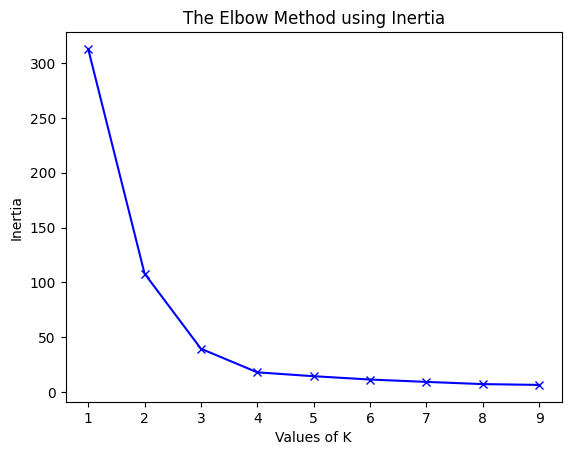
\includegraphics[width=0.4\textwidth]{img/elbow_method.png}
            \caption{Plot of inertia. Possibly good values for $K$ are around 3}
        \end{figure}

        The Silhouette score can also be used by selecting the $K$ corresponding to its maximum.
        Note that, compared to inertia, Silhouette is computationally more expensive.

    \item[Properties] \phantom{}
        \begin{description}
            \item[Termination] 
                There are a finite number of ways to cluster $N$ objects into $K$ clusters.
                By construction, at each iteration, the \texttt{distortion} is reduced.
                Therefore, k-means is guaranteed to terminate.

            \item[Non-optimality] 
                The solution found by k-means is not guaranteed to be a global best.
                The choice of starting points heavily influences the final result. 
                The starting configuration is usually composed of points distant as far as possible.

            \item[Noise]
                Outliers heavily influence the clustering result. Sometimes, it is useful to remove them.

            \item[Complexity]
                Given a $D$-dimensional dataset of $N$ points,
                running k-means for $T$ iterations to find $K$ clusters has complexity $O(TKND)$.
        \end{description}
\end{description}



\section{Hierarchical clustering}

\begin{description}
    \item[Dendrogram] \marginnote{Dendrogram}
        Tree-like structure where the root is a cluster of all the data points and 
        the leaves are clusters with a single data point.

    \item[Agglomerative] \marginnote{Agglomerative} 
        Starts with a cluster per data point and iteratively merges them (leaves to root).
        Uses cluster separation metrics.

    \item[Divisive] \marginnote{Divisive} 
        Starts with a cluster containing all the data points and iteratively splits them (root to leaves).
        Uses cluster cohesion metrics.

    \item[Cluster separation measures]
        Measure the distance between two clusters $K_i$ and $K_j$.
        \begin{descriptionlist}
            \item[Single link] \marginnote{Single link}
                Minimum distance of the points in the two clusters:
                \[ \texttt{sep}(K_i, K_j) = \min_{\vec{x} \in K_i, \vec{y} \in K_j} \texttt{dist}(\vec{x}, \vec{y}) \]
                Tends to create larger clusters.
    
            \item[Complete link] \marginnote{Complete link}
                Maximum distance of the points in the two clusters:
                \[ \texttt{sep}(K_i, K_j) = \max_{\vec{x} \in K_i, \vec{y} \in K_j} \texttt{dist}(\vec{x}, \vec{y}) \]
                Tends to create more compact clusters.
        
            \item[Average link] \marginnote{Average link}
                Average distance of the points in the two clusters:
                \[ \texttt{sep}(K_i, K_j) = \frac{1}{\vert K_i \vert \cdot \vert K_j \vert} \sum_{\vec{x} \in K_i, \vec{y} \in K_j} \texttt{dist}(\vec{x}, \vec{y}) \]
            
            \item[Centroid-based] \marginnote{Centroid-based}
                Distance between the centroids of the two clusters.

            \item[Ward's method] \marginnote{Ward's method}
                Let $K_m$ be the cluster obtained by merging $K_i$ and $K_j$.
                The distance between $K_i$ and $K_j$ is determined as:
                \[ \texttt{sep}(K_i, K_j) = \texttt{SSE}(K_m) - \big( \texttt{SSE}(K_i) + \texttt{SSE}(K_j) \big) \]
        \end{descriptionlist}
\end{description}


\subsection{Agglomerative clustering}

\begin{description}
    \item[Algorithm] \marginnote{Agglomerative clustering} \phantom{}
        \begin{enumerate}
            \item Initialize a cluster for each data point.
            \item Compute the distance matrix between each cluster.
            \item Merge the two clusters with the lowest separation, 
                drop their values from the distance matrix and add a row/column for the newly created cluster.
            \item Go to point 2. if the number of clusters is greater than one.
        \end{enumerate}

        After the construction of the dendrogram, a cut \marginnote{Cut} can be performed at a user-defined level.
        A cut near the root will result in few bigger clusters.
        A cut near the leaves will result in numerous smaller clusters.
        

    \item[Properties] \phantom{}
        \begin{description}
            \item[Complexity] 
                Space complexity of $O(N^2)$ to store the distance matrix.
                
                Time complexity of $O(N^3)$ ($O(N)$ iterations with a $O(N^2)$ search for the pair to merge and $O(N)$ to recompute the distance matrix) 
                that can be reduced to $O(N^2\log(N))$ when using indexing.
        \end{description}
\end{description}



\section{Density-based clustering}

Consider as clusters the high-density areas of the data space.

\begin{description}
    \item[Grid-based] 
        Split the data space into a grid and count the number of points in each tile.

    \item[Object-centered] 
        Count, for each point, the number of neighbors within a radius.
\end{description}


\subsection{DBSCAN}

\begin{description}
    \item[Neighborhood] \marginnote{Neighborhood}
        Given a radius $\varepsilon$, the neighborhood of a point $\vec{x}$ are the points within an $\varepsilon$-sphere centered on $\vec{x}$.

    \item[Core point] \marginnote{Core point}
        Given a minimum number of neighbors $m$, 
        a point $\vec{x}$ is a core point if it has at least $m$ neighbors.

    \item[Border point] \marginnote{Border point}
        A point $\vec{x}$ is a border point if it is not a core point.

    \item[Directly density reachable] \marginnote{Directly density reachable}
        A point $\vec{p}$ is directly density reachable from $\vec{q}$ iff:
        \begin{itemize}
            \item $\vec{q}$ is a core point.
            \item $\vec{q}$ is a neighbor of $\vec{p}$.
        \end{itemize}

    \item[Density reachable] \marginnote{Density reachable}
        A point $\vec{p}$ is density reachable from $\vec{q}$ iff:
        \begin{itemize}
            \item $\vec{q}$ is a core point.
            \item There exists a sequence of points $\vec{s}_1, \dots, \vec{s}_z$ such that:
            \begin{itemize}
                \item $\vec{s}_1$ is directly density reachable from $\vec{q}$.
                \item $\vec{s}_{i+1}$ is directly density reachable from $\vec{s}_i$.
                \item $\vec{p}$ is directly density reachable from $\vec{s}_z$.
            \end{itemize}
        \end{itemize}

    \item[Density connected] \marginnote{Density connected}
        A point $\vec{p}$ is density connected to $\vec{q}$ iff there exists a point $\vec{s}$ 
        such that both $\vec{p}$ and $\vec{q}$ are density reachable from $\vec{s}$.

    \item[Algorithm] \marginnote{DBSCAN}
        Determine clusters as maximal sets of density connected points.
        Border points not density connected to any core point are labeled as noise.

        In other words, what happens is the following:
        \begin{itemize}
            \item Neighboring core points are part of the same cluster.
            \item Border points are part of the cluster of their nearest core point neighbor.
            \item Border points without a core point neighbor are noise.
        \end{itemize}

    \item[Properties] \phantom{}
        \begin{description}
            \item[Robustness]
                Able to find clusters of any shape and detect noise.

            \item[Hyperparameters]
                Sensible to the choice of the radius $\varepsilon$ and minimum neighbors $m$.

                \begin{description}
                    \item[K-distance method] \phantom{}
                        \begin{enumerate}
                            \item Determine for each point its $k$-distance as the distance to its $k$-nearest neighbors.
                            \item Sort the points by decreasing $k$-distance and plot them.
                            \item Use as possible $\varepsilon$ the values around the area where the slope decreases (similarly to the elbow method).
                        \end{enumerate}
                \end{description}

            \item[Complexity]
                Complexity of $O(N^2)$, reduced to $O(N \log N)$ if using spatial indexing.
        \end{description}
\end{description}


\subsection{DENCLUE}

\begin{description}
    \item[Kernel density estimation] \marginnote{Kernel density estimation}
        Statistical method to estimate the distribution of a dataset through a function.

        \begin{description}
            \item[Kernel function] \marginnote{Kernel function}
                Symmetric and monotonically decreasing function to describe the influence of a data point on its neighbors.

                A typical kernel function is the Gaussian.

            \item[Overall density function]
                The overall density of the dataset is obtained as the sum of the kernel function evaluated at each data point.

                \begin{figure}[H]
                    \centering
                    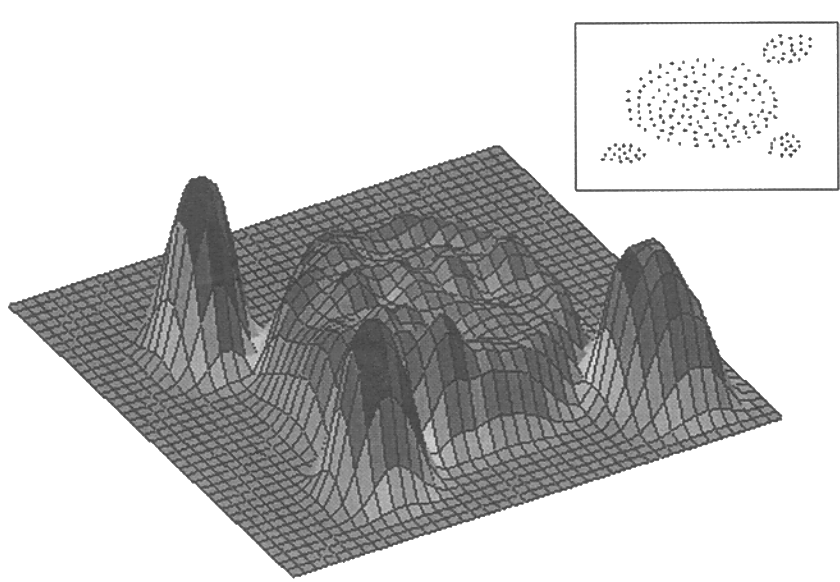
\includegraphics[width=0.35\textwidth]{img/kernel_density_estimation.png}
                    \caption{Example of density function from a set of points (top right) using a Gaussian kernel}
                    \label{img:denclue}
                \end{figure}
        \end{description}

    \item[Algorithm] \marginnote{DENCLUE}
        Given a threshold $\xi$, DENCLUE works as follows:
        \begin{enumerate}
            \item Derive a density function of the dataset.
            \item Identify local maximums and consider them as density attractors.
            \item Associate to each data point the density attractor in the direction of maximum increase.
            \item Points associated with the same density attractor are part of the same cluster.
            \item Remove clusters with a density attractor lower than $\xi$.
            \item Merge clusters connected through a path of points whose density is greater or equal to $\xi$ 
                (e.g. in \Cref{img:denclue} the center area will result in many small clusters that can be merged with an appropriate $\xi$).
        \end{enumerate}

    \item[Properties] \phantom{}
        \begin{description}
            \item[Robustness]
                Able to recognize clusters of different shapes and handle noise.

            \item[High dimension weakness]
                Does not perform well with high-dimensional data with different densities.

            \item[Complexity]
                Computational complexity of $O(N^2)$.
        \end{description}
\end{description}



\section{Model-based clustering}

Assuming that the attributes are independent random variables,
model-based clustering finds a set of distributions (one per cluster) that describe the data.


\subsection*{Gaussian mixture (expectation maximization)}

\begin{description}
    \item[Algorithm] \phantom{} \marginnote{Gaussian mixture} 
    \begin{enumerate}
        \item Select an initial set of parameters for the distributions.
        \item Expectation step: for each data point, compute its probability to belong to each distribution.
        \item Maximization step: tweak the parameters to maximize the likelihood (i.e. move the Gaussian towards the center of the cluster).
        \item Go to point 2. until convergence.
    \end{enumerate}
\end{description}